
\documentclass{article}
\usepackage{spconf,amsmath,graphicx}
\usepackage[obeyspaces]{url}

\def\x{{\mathbf x}}
\def\L{{\cal L}}


\title{COMP421(2020T2) - Final Project Report}

\name{Au Tsz Kin}
\address{Victoria University Wellington}


\begin{document}

\maketitle

%\begin{abstract}
%TBA
%\end{abstract}

\section{Introduction}
\label{sec:intro}

In this report, we explore the unsupervised anomaly detection technique using
Long short-term memory(LSTM) in temporal data, which LSTM is a variant of
recurrent neural networks (RNNs). Akash Singh's master thesis
\cite{7-lstmthisis} is selected to best suit the
subject, there were discovery and improvement made around his LSTM RNN
model.

The original code can be found in \cite{7-lstmthisis}. And the modified code is
stored in my GitHub repository and can be downloaded and viewed publically:
[\url{https://github.com/AUTSZKIN/COMP421-Final-Project}]

\subsection{Anomaly Detection}
Anomaly detection is a significant problem that has been studied within
a wide variety of research areas and application domains. It refers to the
problem of finding patterns or instances in data that do not match to expected
behaviour. These deviated patterns or instances can be described as
anomalies, outliers, exceptions, aberrations, surprises, peculiarities,
discordant observations, or contaminants depending on domain and context
\cite{1-Anomalydetection}. Anomaly detection is useful and significant as
the detected anomalies in data often translate to significant, actionable,
or even critical information in various application domains. For example,
anomaly detection
techniques can be used in life-critical systems to detect faults, invasion
detection for
cyber-security, fraud detection for credit cards, insurance, or other
finance-related areas. 

\subsubsection{Challenges of anomaly detection}
The definition of anomalies is different across application domains. In the
real-world, defining a region of data that include every variation of normal
behaviour is not easy; critical anomalies that lie on the edge of the border
can be considered normal, thus cause false-positive errors or vice versa. 

Anomaly detection is usually considered an unsupervised problem,
because anomalies are rare and often not seen before; when new
samples arise or system update required, a new type of anomaly might come
along, therefore it is impossible to define every variation of an anomaly in
advance.
Annotating anomalies is often a time-consuming process and domain experts
with sufficient knowledge are required to label anomalies. We are performing
anomaly detection on time series data in this report,
there will be more challenges involved, QIANG YANG
et al. \cite{2-10challengingproblems} stated that time-series data remains it
own problem,  a large variety of time series used for predictions are
contaminated by noise, that makes a prediction on short-term and
long-term more difficult.

%\textit{ The terms "anomaly/anomalies" were used to
%refer to the patterns or instances that deviated from the normal pattern in
%dataset used. }


\subsection{Recurrent Neural Network (RNN)}

Recurrent Neural Network(RNN) is a class of artificial neural networks that
allow previous outputs to be used as current inputs
while having hidden states; therefore having the ability to learn long-term
temporal patterns. RNNs are unlike Fully-Connected Networks or Convolution
Networks, which lack "memories" when processing sequences or time series of
data (e.g. climate data, stock market, medical data). In reality,
when we understand the meaning of a sentence, each word is not independent, and
we also have its context in our minds. Therefore the basic concept of RNN is to
maintain some intermediate state information to help understand the
context. RNN models are mostly used in the fields of
natural language processing and speech recognition. 

Fig.\ref{fig: RNN} shows a vanilla RNN, hidden units grouped with state $s$ at
time $t$, each neuron receive inputs from previous neurons at time step $t-1$,
and passing the output to the next neuron at $t+1$, the state vector is
preserved during its forward computation. 

\begin{figure}[htb]
    \centering
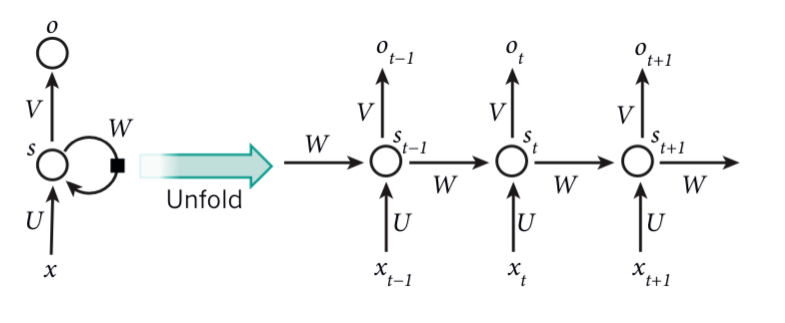
\includegraphics[scale=0.24]{png/RNN.png}
    \caption{A vanilla RNN, image used from \cite{3-deeplearning}}
    \label{fig:RNN}
\end{figure}


\subsubsection{Limitation} 
Training RNNs has proved to be difficult because the backpropagated gradients
either grow or shrink at each time step, so when process sequences
that are very long, RNN is prone to problems such as gradient exploding and
gradient vanishing\cite{3-deeplearning}. 

\subsection{Long Short-Term Memory (LSTM) }

Long Short-Term Memory (LSTM) is a variant of RNN, it was introduced in
\cite{4-lstm}, it has been proved to be a better successor of RNN in learning
long-range temporal data, it
mainly solved the vanishing gradients problem during long sequence training in
RNN.
Simply put, compared to vanilla RNNs, LSTM can perform better in learning
long-term dependencies. Other than allowing previous outputs to be used as
current
inputs while having hidden
states in RNN. LSTM adds a method that can transmit information with multiple
timesteps apart. Think of a conveyor belt/carry track running together when you
process the sequences. The information of each node in sequence can be put on
the conveyor belt, or taken off from the conveyor belt, of course, you can also
update the information on the conveyor belt. In this way, the information long
ago is preserved and the loss of information is prevented.

To be exact, the main units of LSTM are introduced in \cite{4-lstm} and
\cite{5-forgetgate} and the illustrative diagram of a LSTM unit is shown in
Fig.\ref{fig:forgetgate} :
\begin{itemize}
	\setlength{\itemsep}{1pt}
	\setlength{\parskip}{0pt}
	\setlength{\parsep}{0pt}
  \item A central unit called Constant error carousel (CEC), which allows for
constant error flow
through special self connected units.
  \item Three gates/multiplicative units that control the flow in CEC;
  \begin{itemize}
 		\item Input gate: prevents CEC from receive irrelevant inputs; 
		\item Forget gate: the mechanism is introduced in \cite{5-forgetgate} that
allow LSTM to "forget" or abandon old and no longer relevant content in
memory.
 		\item Output gate prevents other units receive disturbing information from
CEE;
	\end{itemize}
\end{itemize}


\begin{figure}[htb]
	    \centering
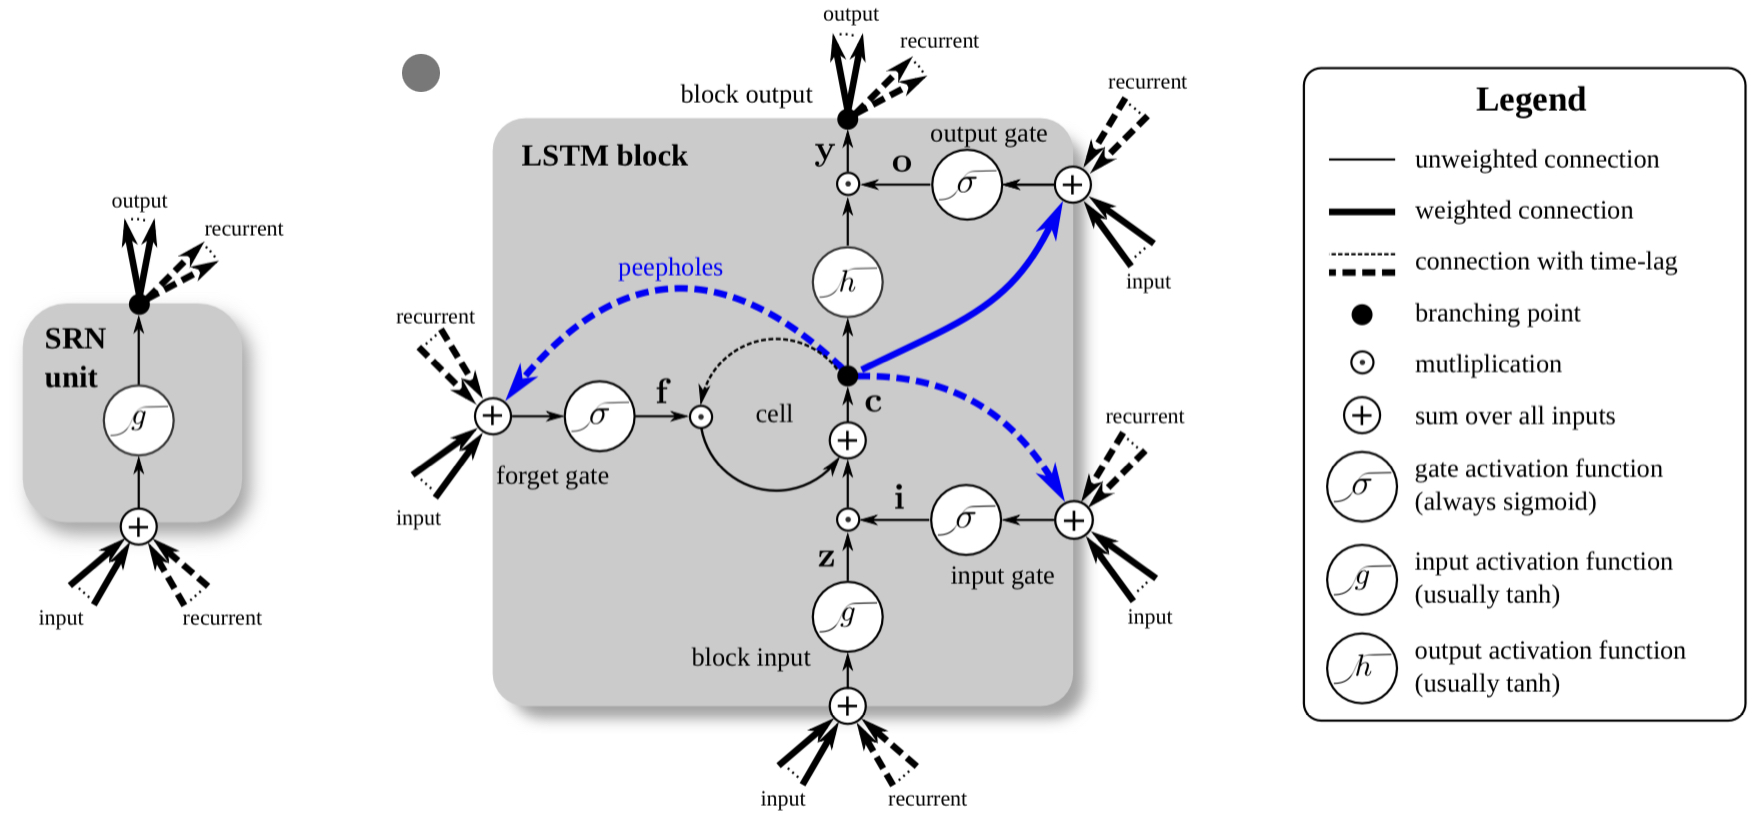
\includegraphics[scale=0.142]{png/forgetgate.png}
    \caption{LSTM with forget gate compare with a simple recurrent network
(SRN), image used from \cite{6-forgetgategraph}}
    \label{fig:forgetgate}
\end{figure}


\subsection{Selected Paper}

The suitable paper selected to match the subject is Akash Singh's master thesis
\cite{7-lstmthisis}. He is an ML Engineer/Data Scientist; Master in Data
Science
from KTH Information and Communication Technology. He used an unsupervised
approach to accomplish Long short-term memory (LSTM) technique for anomaly
detection in time-series data since the data are unlabelled. 

An RNN model with LSTM units was trained to learn the normal temporal patterns
and predict values in future time steps. The anomaly scores are given by
modelling prediction error result; therefore determine whether an instance is
an
anomaly or not. Singh also explored different ways to maintain state in LSTM
and the effect of the different number of time steps used on prediction and
detection performance.

Three real-world datasets were used in his experiments, the results show that
maintaining the LSTM state is critical for getting a proper result, LSTM RNNs
are
suitable for general purpose time series modelling and anomaly detection.

\subsection{Contribution}

TBA 

\section{Methods, Network Architecture, Datasets and File Directories}

Singh's experiments and model \cite{7-lstmthisis} was written and
implemented using Python
programming language with Keras; His algorithm contains two parts. Part one is
to train a prediction model by learning normal temporal patterns from the
dataset,
the model can predict future time series. Part two is the anomaly detection,
anomaly scores are computed from the prediction errors.


\subsection{Prediction Model}
The term $lookback$ number and $lookahead$ number were used in 
the model as input the most recent $p$ value and output $q$ value respectively.

The network contains hidden recurrent layer/layers followed by an output
layer. The number of hidden recurrent layers and units varies for different
datasets. Two recurrent layers are fully connected with each other. To avoid
overfitting $dropout$ is used between two recurrent layers. The output layer is
a fully connected dense NN layer. The number of neuron nodes in the output
layer is equal to the $lookahead$ value, with one neuron for each future value
predicted. Since the model is used for regression, linear activation is used in
the output layer and mean-square error(MSE) as the loss function
\cite{7-lstmthisis}.

The main purpose of the prediction model is to predict multiple time steps
ahead, that is, predicting multiple future values; With a $lookahead$ of $q$ at
time $t$ the model predicts the next $q$ future values i.e.
$t$+1, $t$+2..., $t$+q. Consider a time series with a scale of 10 minutes.
Predicting $lookahead$ value of 6 can give us the behaviour
of the time series for the next 30 minutes. It is useful for a system to
predict
possible unusual behaviour, e.g. an extreme value, early alerts can be sent
out. 

\subsection{Anomaly Detection and Data Pre-processing}
The prediction errors are used as anomaly indicators, which
is the difference between prediction made at time step $t$-1 and the input
value received at current time step $t$. The prediction errors from training
data are modelled using a Gaussian distribution; the mean and variance are
computed using maximum likelihood estimation (MLE). 

On new data, the log probability densities (PDs) of errors are calculated and
used as anomaly scores: the lower the PD values the greater likelihood of the
instance being an anomaly. A validation set contains both normal instances and
anomalies are used to set a
threshold on log PD values; it can separate anomalies from normal
instances and produce as few false-positive errors as possible. Finally, a
separate test set containing both normal instances and anomalies is used to
evaluate the model.

In order to learn normal time series patterns and optimise prediction
performance, only normal data without anomalies is used for training LSTM RNN
model. For the different dataset, each is divided into four subsets: a training
set, $N$, with only normal values; validation set, $V_N$, with
only
normal values; a second validation set, $V_A$, with
normal values and anomalies; and a test set, $T$, having both normal values
and anomalies.
There are three main procedures of the LSTM RNN training algorithm:
\begin{itemize}
	\setlength{\itemsep}{1pt}
	\setlength{\parskip}{0pt}
	\setlength{\parsep}{0pt}
	\item 1. Set $N$ with only normal values is used for training prediction
model, Bayesian optimization \cite{8-BayesianOp} to find the best values
for network hyper-parameters. And $V_N$ is used for early stopping to prevent
model overfitting.
	\item 2. Gaussian distribution is used for modelling prediction errors on $N$.
The trained prediction model is applied to $V_A$. The log PD of errors are
calculated from $V_A$ and used as anomaly scores. A threshold is set on the log
PD values which separate the possible anomalies from normal values.
	\item 3. The prediction errors from the test set $T$ is used for the set
threshold, therefore it is used as an anomaly indicator to identify anomalies
from
the test set $T$.
\end{itemize}

\subsection{Datasets}
It is difficult to judge how well an anomaly detection algorithm
would generalize to different type datasets and there is no real-world validity
of the actual anomalies and algorithm performance if artificial
datasets are used to train the model \cite{7-lstmthisis}. 

Therefore instead of using application-specific datasets or artificial
datasets, three real-world data sets were used in Singh's experiments:
Numenta’s MachineTemperature Dataset, Power Demand Dataset and ECG Dataset. All
three datasets contain real-world anomalies annotated by domain experts and all
been used in previous works on anomaly detection.


\subsection{Code Directories}
The full code of the project is under \path{/Code}. There are 5 main parts
of the original code that I explored or conduct experiments.

\begin{itemize}
	\setlength{\itemsep}{1pt}
	\setlength{\parskip}{0pt}
	\setlength{\parsep}{0pt}
	\item The configuration of model hyper-parameters is placed under
\path{/Code/configuration/}
	\item The real-world datasets are stored in \path{Code/resources/data/}
	\item The LSTM model implementation is placed under \path{Code/models/}
	\item The LSTM predictor that train model and predict results is
\path{Code/lstm_predictor.py}
	\item The data pre-processing and anomaly detection are executed by using
Python Notebook, the notebooks are under \path{Code/notebooks/}
\end{itemize}


\section{The Issues of Current System}

Singh's model is worked quite well for both Power Demand Dataset and
ECG Dataset (i.e. the electrical activity of the heart). According to Singh's
thesis, the model detected all 5 anomalies in the Power Demand test set with
the PD threshold of $-24$ but there is 1 small false-positive error. For ECG
test
set, the model with a threshold of $-23$ detects all three anomalies with no
error. It is because they all have consistent and repetitive patterns and the
LSTM model will be relatively easy to learn these pattern.
Fig.\ref{fig:powerdemand} shows example plots of a normal and an anomalous
weekly cycle, the ECG dataset is produced the plot similar to Power Demand
Dataset.

\subsection{Problem of the machine temperature dataset}

There are four anomalies in the machine temperature
dataset distributed in the sets $V_A$ and $T$ (See
Fig.\ref{fig:actualAnomalies}), the results of the anomaly
detection on $V_A$ and $T$ are shown in
Fig.\ref{fig:o-validationResult} and Fig.\ref{fig:o-testResult} respectively;
Orange shaded area in the graph denotes possible anomalies made by the LSTM
algorithm. 

\subsubsection{Results}
\label{originalresults}
\begin{itemize}
	\item For the validation set $V_A$: The PD threshold of $-11$ was necessary to
detect the first anomaly in set $V_A$, but there are quite a few false
positives errors, see Fig.\ref{fig:o-validationResult}.
	\item For the test set $T$: On $T$ the threshold of $-11$ detected the second
anomaly but did not detect the first anomaly, and also incurred quite a lot
false-positive errors before the first anomaly and around the second anomaly
see
Fig.\ref{fig:o-testResult}.
\end{itemize}

The detection result of the machine temperature dataset is not as good as the
previous two. Since the machine temperature dataset does not seem to have any
repeating pattern, so the model did not maintain LSTM state between
batches. And indeed the performance of the Singh's model was found to be
insensitive to how the state was maintained as he mentioned on the thesis.
The result with too many false positives is making the detection
system unusable.

\subsubsection{Original model architecture}
\label{originalmodel}
The LSTM RNN model Singh used for the machine temperature
dataset prediction and anomaly detection had a $lookback$ of 24, a $lookahead$
of 12, two hidden recurrent layers with 80 and 20 LSTM units respectively, a
dense output layer with 12 neurons, and a dropout of 0.1.  With Adam optimizer
using a learning rate of .05, a decay of
0.99, and a batch size of 1024. The training was done for 200 epochs with early
stopping. This model gave an MSE of 0.09 on $N$.
Using set $V_A$ a threshold of $-11$ was set on the log PD values. The
threshold was then evaluated using set T.

\subsection{Effect of lookback value}
\label{lookbackeffect}
The parameter $lookback$ is an important parameter that
affects learning, it is the number of time steps for which the RNN is
unfolded for back-propagation. Singh found that there is no
general optimal value of $lookback$ in Section 4.4.1 \cite{7-lstmthisis};
$Lookback$ value depends on the characteristic of data and the temporal
correlations present in it. Lookback values ranging from 8 to 200 have been
used successfully for different tasks. Which Singh discovery on $lookback$ is
verified by my experiment. 

However, the selected $lookback$ value of 24 in Singh's original machine
temperature dataset model does not seem to be the best choice; In my
experiment, I have discovered that the $lookback$ of 50 produced a better
prediction result than Singh's result which is discussed further in Section
\ref{experiment}.

\subsection{Trade-off between Prediction Accuracy and Anomaly Detection}
\label{tradeoff}
Singh stated in Section 4.4.2 \cite{7-lstmthisis} that he experienced a
trade-off between prediction performance and the results of anomaly detection.
An LSTM RNN model optimised for minimising the prediction MSE was not the best
for anomaly detection. The prediction errors were small throughout the set
$V_A$ and $T$ making it difficult to find a good PD threshold to split
anomalies from normal values without incurring too many false positives.
This is the same result as described in Section \ref{originalresults}.

But Singh's conclusion of the trade-off between Prediction
Accuracy and Anomaly Detection does not seem valid; I have conducted a series
of tests to improve the prediction accuracy while gaining a better anomaly
detection result at the same time, which proved the invalidity of his argument.
This is discussed in the next section.


\section{Experiment Result and Contribution}
\label{experiment}

On the machine temperature dataset, Singh's model did not perform as desired as
the other two; As the machine temperature dataset contains inconsistent
patterns, the model is difficult to maintain LSTM state between batches. 

Also, Singh's arguments in Section \ref{lookbackeffect} and Section
\ref{tradeoff} is rather weak and vague, or there is no definite proof to
support it. So the content of the following experiment is inspired by Singh's
arguments. The goal of the experiment is to improve the prediction accuracy
while achieving a better result of anomaly detection on the machine temperature
dataset, if not worse than the existing one. 

\subsection{The result from Singh's LSTM RNN model}
\label{originalmodelresult}
The original architecture with 24 $lookback$ described in Section
\ref{originalmodel}; In my experiment, Singh's model which gave us MSE of
0.089 on the Training set ($N$), this is very consistent with his results. The
Validation ($
V_A)$ Loss is 1.30 and the Test Loss ($T$) is 0.347

\subsection{Change the lookback value}

There is one figure of training MSE on ECG dataset for different values
of $lookback$, but none for the power demand dataset nor the machine
temperature dataset; There is no detail about how different values of
$lookback$ are been used in the original model. From this point of view, one
possible way to improve the performance on the machine temperature dataset is
to test different $lookback$ values.
\textit{The training and result log can be viewed under
\path{Code/logs/0-original-model-24lookbacks.log} }

\subsubsection{Experiment steps}

Test with various hyperparameter candidates to train model to get
desired/better result. All the results are stored in \path{Code/logs/}
\begin{itemize}
	\setlength{\itemsep}{1pt}
	\setlength{\parskip}{0pt}
	\setlength{\parsep}{0pt}
	\item Test didffernt value of $lookback$
		\begin{itemize}
			\item From 10-300, with interval of 10, test each $lookback$ value on the
original model, but change the lookahead value to 1 to decrease the training
time.
			\item The training and result log can be viewed under
\path{Code/logs/1-lookback-10to300-run.log}
		\end{itemize}
	\item The best $lookback$ candidates are $[50, 60 and 150]$, each were tested
with epochs of $[20, 40, 80, 160 and 320]$. 
		\begin{itemize}
			\item Similarly, 50 $lookback$ trained with 320 epochs gave us the best
result, $N$ MSE: 0.017, $V_A$ Loss:0.40 and $T$ Loss: 0.045. It is because the
$lookahead$ value is set to 1, therefore the result will have much higher
prediction accuracy than the one with the$lookahead$ set to 12.
			\item The training and result log can be viewed under
\path{Code/logs/2-find-best-lookbacks.log}
		\end{itemize}
	\item Then I used $lookback$ value of 50 instead of 24 in the original model
architecture described in Section \ref{originalmodel}:
		\begin{itemize}
			\item The result showing: $N$ MSE: 0.0867, $V_A$ Loss:0.39 and $T$ Loss:
0.22; Comparing the result from Singh's model in Section \ref{originalresults}.
The improvement of using 50 $lookback$ is noticeable.
			\item The training and result log can be viewed under
\path{Code/logs/3-final-modified-model}
		\end{itemize}
\end{itemize}

\subsection{Result after using 50 as the lookback value}

Singh argued that increasing $lookback$ values improved prediction performance
up to a limit and no improvement was gained by increasing the lookback values
further, which show to be true by my experiment; 200 or 300 $lookback$ did not
produce a better result than 50 $lookback$ did. However, according to my
experiment result, Singh's choice of selecting 24 as the optimal $lookback$ for
the machine temperature dataset is proved is not the best. 

The Validation and Test sets results of the final model using 50 $lookback$ is
shown in Fig.\ref{fig:m-validationResult} and Fig.\ref{fig:m-testResult}; My
model is similar to Singh's. The two anomalies in $V_A$ and the second anomaly
in $T$ are found, but the first anomaly in $T$ is not detected. Having said
that, compare my results with the original results in
Fig.\ref{fig:o-validationResult} and Fig.\ref{fig:o-testResult}, we can see
the prediction accuracy is observable higher: the predicted value (green dot
line) is better fit the true value (blue line) than the original ones; And the
error (red line) is lower than the original ones as well, especially at the
spot of the second anomaly in the Validation sets.

Not only the prediction accuracy of my model out-rated the original one while
found the same anomalies, but it also decreases the anomaly false positive
errors. The Orange shaded area in the graph denotes possible anomalies made by
the LSTM algorithm. Comparing my results (Fig.\ref{fig:m-validationResult} and
Fig.\ref{fig:m-testResult}) with Singh's (Fig.\ref{fig:o-validationResult} and
Fig.\ref{fig:o-testResult}), it is notable that the model after the
modification
has much lesser false-positive anomalies. This result makes Singh's assertion
of
the trade-off between prediction accuracy and anomaly detection to be false. 

\subsection{Other experiments}
I also modified the amount of recurrent layer and LSTM units in it, the
hyper-parameters, architecture, and final results can be viewed in
\path{Code/logs/4-50lookback-2layers.log}, this model also gave us a better
MSE and Loss result. Due to the time constraint, the anomaly detection test
is not been executed, but this gave us the opportunity of the potential
improvement of the LSTM RNN anomaly detection model.

\subsection{Code modified}
The main code I have modified is under
\path{Code/lstm_predictor-modified.py} and
\path{Code/configuration/config_modified.py}


\section{Conclusion}
According to the principle of Occam's razor, I did not do too many changes to
the original model of Singh, but from the basic parameters modify the test to
obtain the desired result. 

Although my model is similar to Singh's but the accuracy of the prediction
model is significantly improved, thereby reducing the error rate of false
positives. This proves that Singh's model has a lot of room for improvement. If
time permits, I believe that the model can be further optimised and can be used
in the real-life systems. My experiments and modification have also proved that
unlike ordinary Feed-forward neural networks or Convolutional neural networks,
for different types of data, there is no unified or generalised LSTM model
structure for anomaly detection; depending on different data types and
characteristic, the appropriate number of hidden recurrent layers, neurons and
suitable hyper-parameters should be tested and used to gain the possible best
result.

%根据奥卡姆剃刀原则,我没有做过多的修改,而是从基本的参数修改测试入手从而得到了期望的结果,
%虽然我的模型与Singh的类似,$V_A$中的两个2个和$T$中的第二个anomaly都找到了,但并没有检测到$T$中的第一个anomaly,
%但是预测模型的准确度显著提高了,从而降低了false positives的错误率. 这证明了Singh的模型有许多提升的空间, 如果时间允许, 
%我相信该模型能被进一步优化而能被现实生活中的系统所使用. 我的实验还证明了,不像普通的神经网络或
%卷积神经网络,对于不同性质的数据,并没有统一或者泛化的用来进行anomaly detection的LSTM模型结构; 根据不同的数据类型,
%应该测试并使用合适数目hidden recurrent layers, neurons和合适的hyper-parameters. 


\clearpage
%\vfill\pagebreak

\begin{figure}[htb]
	    \centering
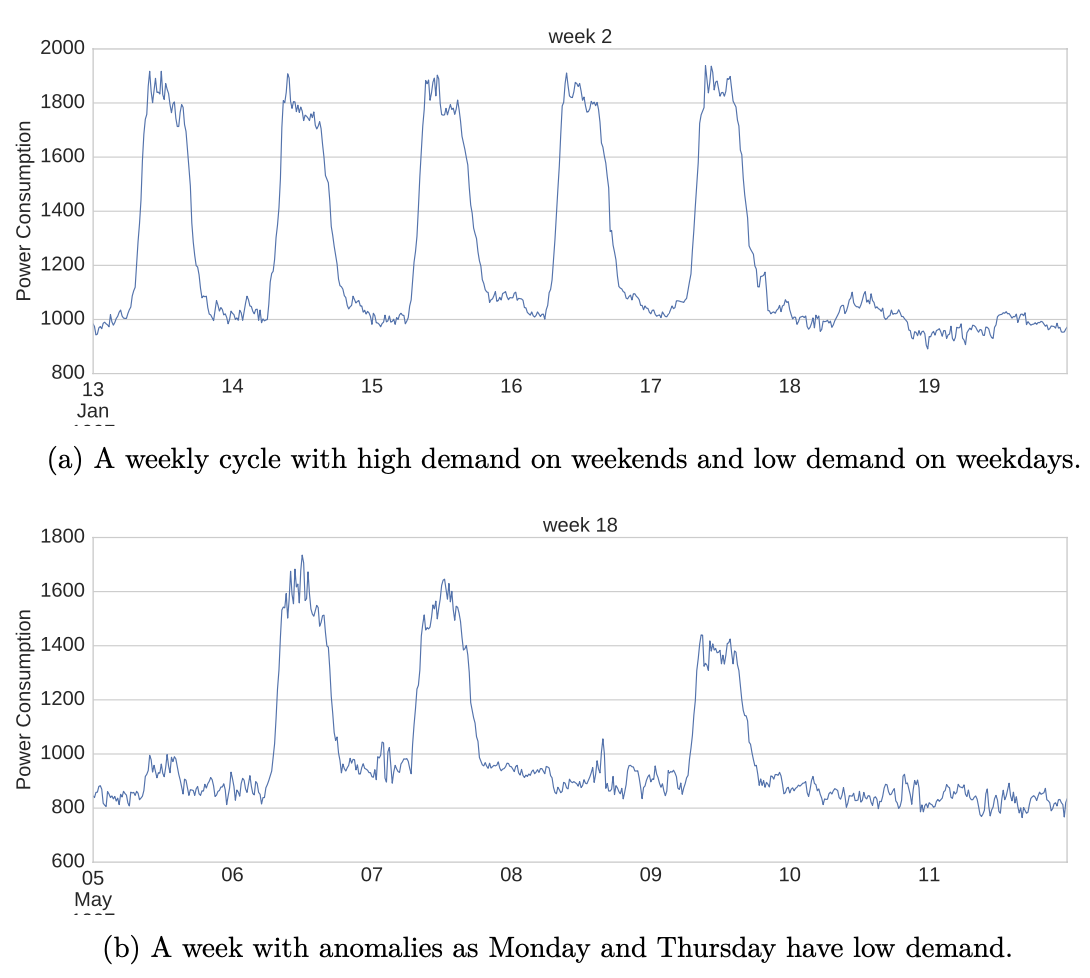
\includegraphics[scale=0.45]{png/powerdemand.png}
    \caption{Power demand normal and anomalous patterns
\cite{7-lstmthisis} }
    \label{fig:powerdemand}
\end{figure}

\begin{figure}[htb]
	    \centering
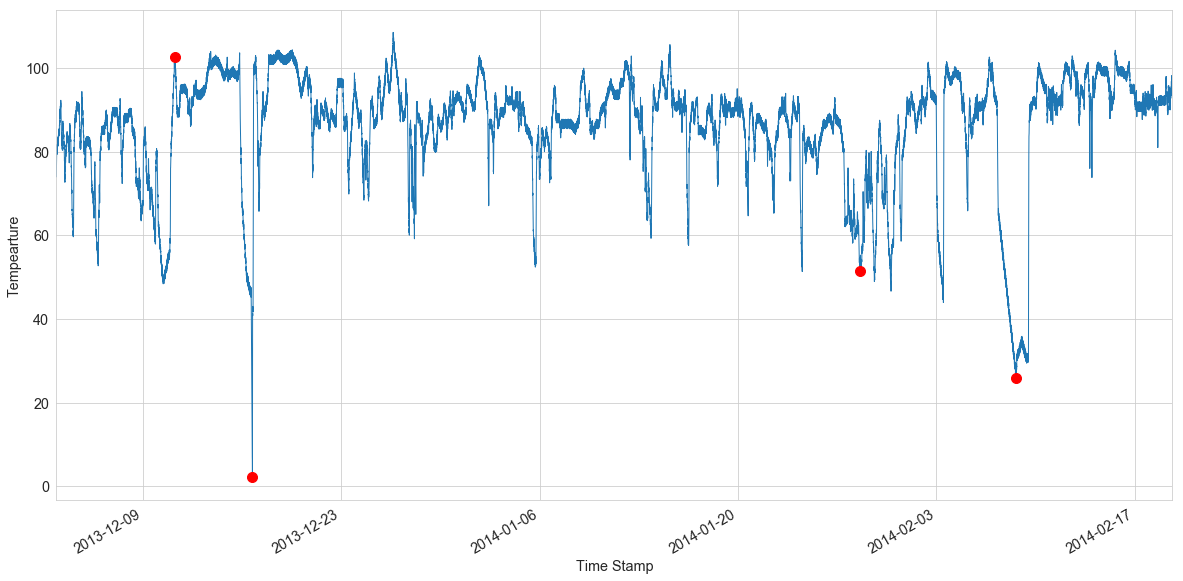
\includegraphics[scale=0.21]{png/o-actualAnomalies.png}
    \caption{Normal pattern/values and actual anomalies in the Numenta’s
Machine Temperature Dataset; Four known anomalies indicated by red markers. The
X-axis shows time steps, and the Y-axis measures temperature}
    \label{fig:actualAnomalies}
\end{figure}

\begin{figure}[htb]
	    \centering
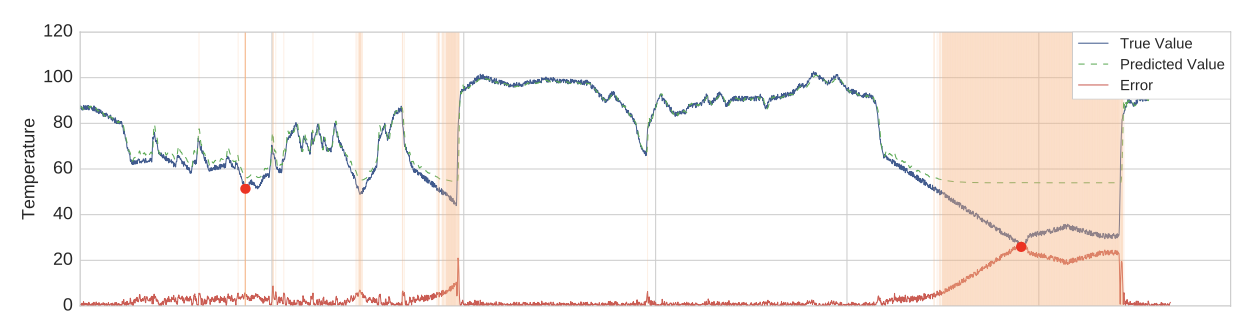
\includegraphics[scale=0.41]{png/o-validationResult.png}
    \caption{Original validation set results on machine temperature dataset. 
The X-axis shows time step. Orange shaded area in the graph denotes possible
anomalies made by the LSTM
algorithm}
    \label{fig:o-validationResult}
\end{figure}

\begin{figure}[htb]
	    \centering
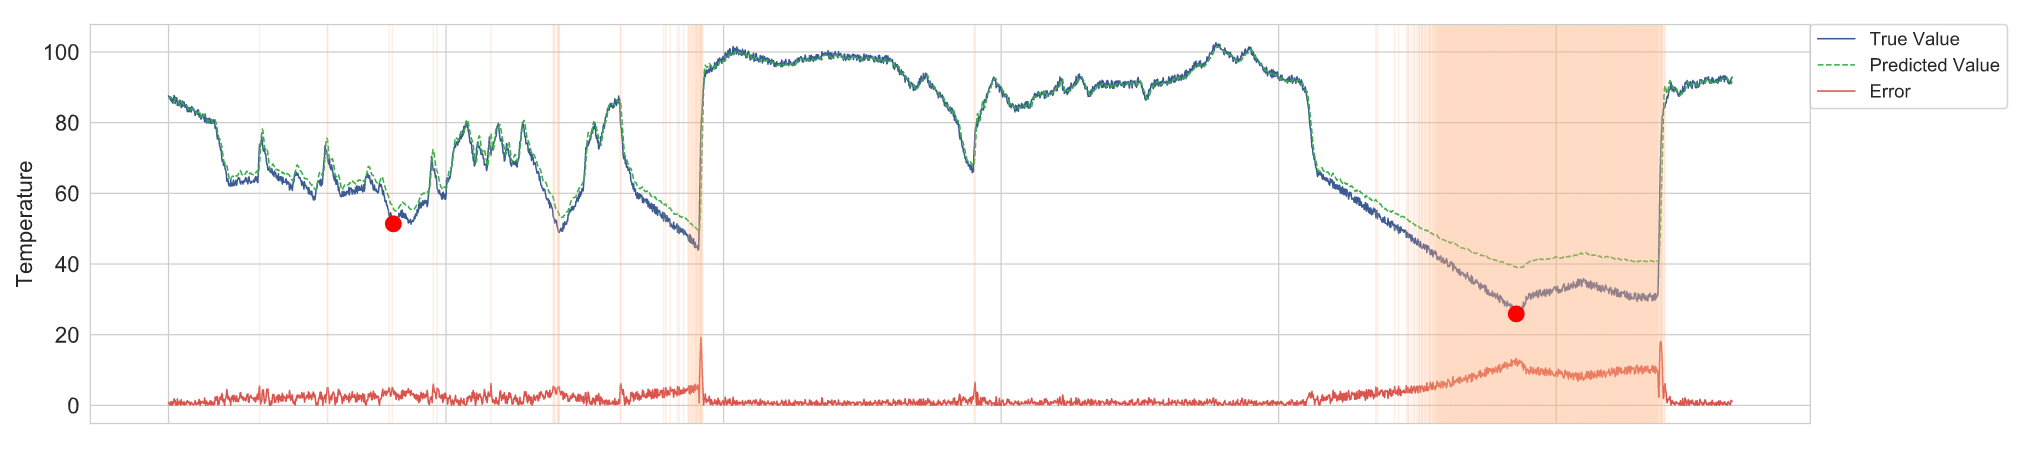
\includegraphics[scale=0.26]{png/m-validationResult.png}
    \caption{Validation set results on machine temperature dataset after
modification}
    \label{fig:m-validationResult}
\end{figure}

\begin{figure}[htb]
	    \centering
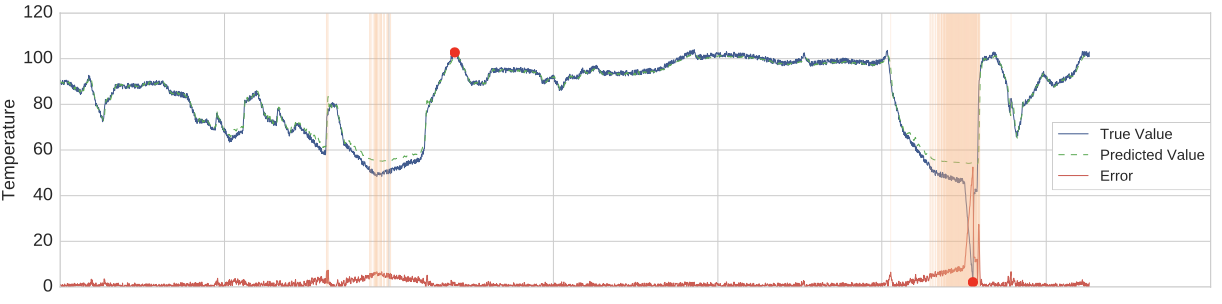
\includegraphics[scale=0.42]{png/o-testResult.png}
    \caption{Original test set results on machine temperature dataset}
    \label{fig:o-testResult}
\end{figure}

\begin{figure}[htb]
	    \centering
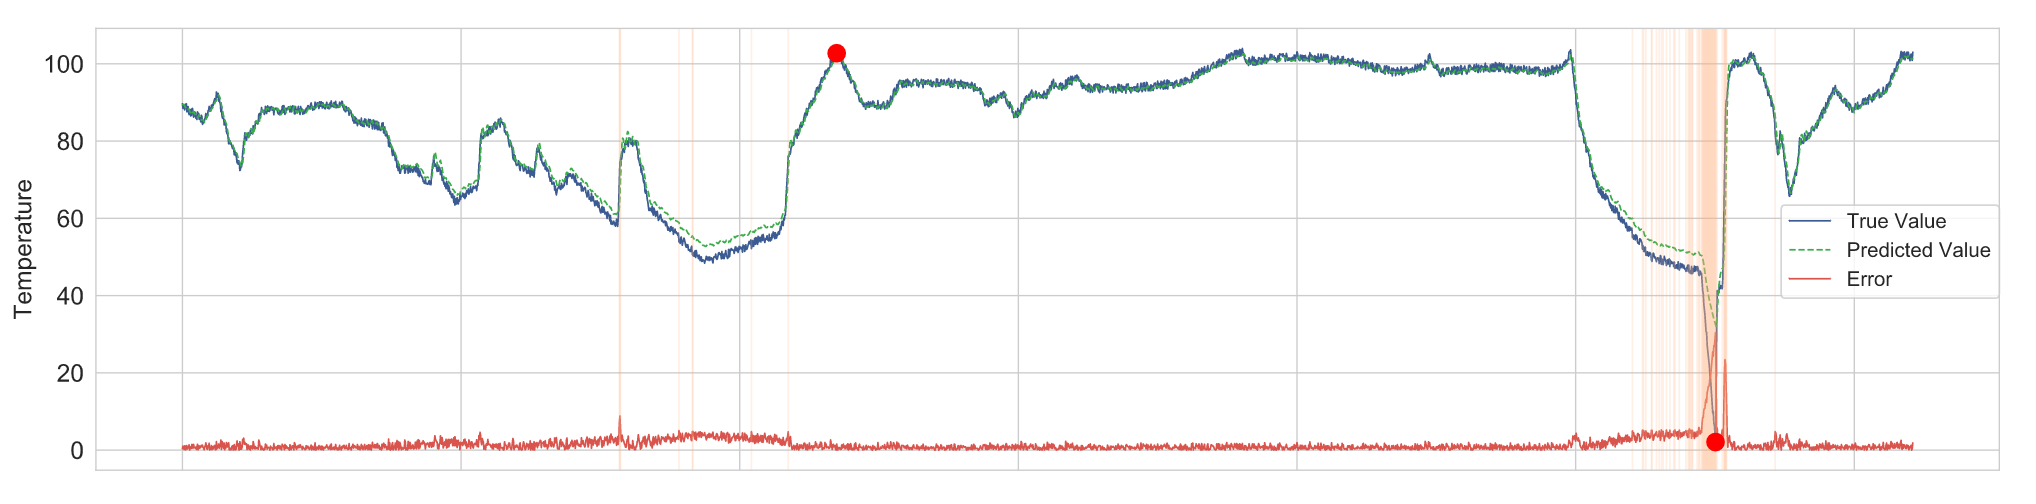
\includegraphics[scale=0.26]{png/m-testResult.png}
    \caption{Test set results on machine temperature dataset after
modification}
    \label{fig:m-testResult}
\end{figure}

\begin{figure}[htb]
	    \centering
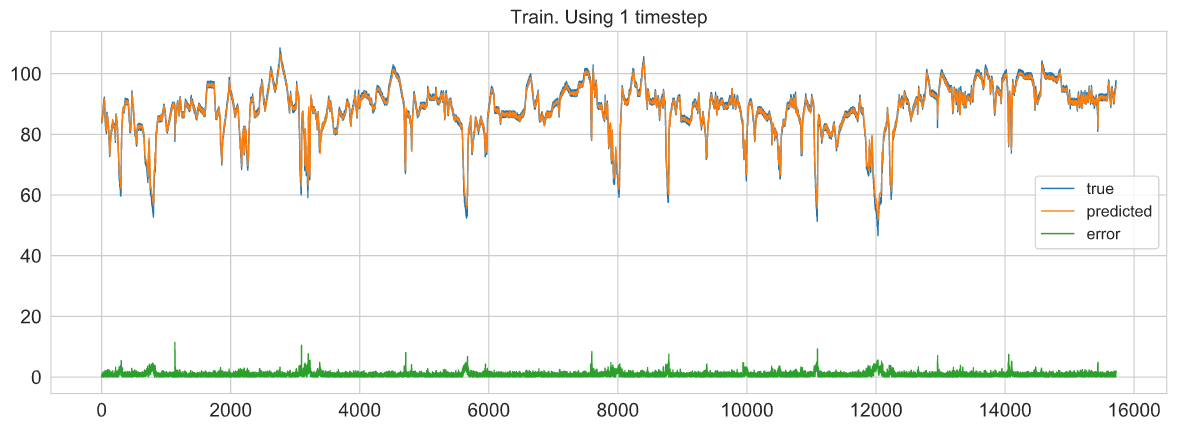
\includegraphics[scale=0.21]{png/m-prediction.png}
    \caption{Prediction result on machine temperature dataset after
modification}
    \label{fig:m-prediction}
\end{figure}

\clearpage


% References should be produced using the bibtex program from suitable
% BiBTeX files (here: strings, refs, manuals). The IEEEbib.bst bibliography
% style file from IEEE produces unsorted bibliography list.
% -------------------------------------------------------------------------
\bibliographystyle{IEEEbib}
\bibliography{refs}

\end{document}
